\section{Definitions and Conventions}\label{theory}
The basic expressions used in this paper are explained in the following chapter. First Representation Learning is defined and the different approaches to find representations of data are explained. A description on how to evaluate the found representations is given. Afterwards Zero Shot Learning as well as Anomaly Detection is described and explained.

% TODO put formulas for a time series and the anomalies. maybe some anomaly score too

\subsection{Representation Learning}
%Intro to RL
% Sensors and comparable applications produce values which vary over time. Sometimes the values vary in an unforeseen way and for a short time window they may be completely random. We have to step back and observe longer time periods.
% Sometimes it is possible for a human to see some patterns in the data when observing a long time window. In the measuring of a solar plant it is obvious that the sun rises and sets, depending on the voltage of the panels. Starting with 0 V at night the voltage is rising before noon, having its peak at midday and descending in the afternoon. This is one representation in the data. But there could be more represenations hidden, which are not likely to see. The shadow of a tree wandering over the panels happening every day or a one time event like the snow covering the plant. \\\\
Variations in data are not always visible for a human and even less possible to label them accordingly. Like \cite{bengio_representation_2013} mentioned it is important for artificial intelligence to detect representations of data by machines. A machine should be able to extract information hidden in the low-level sensor measurings and continue working with the representations instead of the raw data. This is according to the paper the main requirement for a good representation, to be able using it as an input to a supervised predictor.

% What are representations
Representation Learning (RL) tries to detect meaningful interconnections in data relevant for further data analysis. These interconnections represent abstract information, so called background knowledge \cite{lavrac_representation_2021}.

% cognitive representations
In neural networks representations are learned in every layer. The representations in hidden layers are incomprehensible to humans. They are produced by weights and biases and build so called neural representations. At a higher level of abstraction, these neural representations can be understood as spatial representations within a conceptual space, where concepts are represented as points or regions. When these spatial representations are transformed into language, they become symbolic representations, which are used to convey meaning in a human-understandable form. Together, neural, spatial, and symbolic representations build cognitive repesentations \cite{gardenfors_conceptual_2000}.

% Knowledge discovery process
To extract representations a knowledge discovery process with different methods of machine learning and data mining methods are used. During the process representations are learned by the model. RL methods are divided into Propositionalization as symbolic representations and Embeddings as spatial representations \cite[p. 4]{lavrac_representation_2021}.

% RL techniques
RL occurs in several machine learning areas. Depending on the underlying concept, different strategies to extract representations can be found. They work different in detecting patterns and store them in different ways \cite{bishop_pattern_2006}.

% description and main goal
In the book of \cite[p. 525]{goodfellow_deep_2016} a general detailed description of representation learning is given. They summarize that representations should make the subsequent learning tasks easier. This implies that to find the best fitting representation and the underlying representation learning technique, we need to know the task it should perform afterwards.
\subsubsection{Concepts}
% MLP
The most straight-forward approach to detect representations are Multi Layer Perceptrons (MLP). An input vector is processed by interconnected artificial neurons. The neurons build layers starting with an input layer, followed by hidden layers with a final output layer. The produced output layer typically classifies the input and predicts the label. The difference between predicted and labeled output indicates the performance of the network. Adjusting the interconnections using weights and biases of each neuron enables a learning process. \cite{nielsen_neural_2015}

% CNN
Convolutional Neural Networks (CNN) are a variation of the MLP building subsets of the input vector. This is mainly used in image processing.

%RNN
Recurrent neural networks (RNN) are another variation of the traditional feed-forward MLP. Every neuron has an additional input containing the previous state. This is especially useful for time series data.

Traditional neural networks like MLP, RNN, and CNN have limitations in learning robust, generalizable, and semantically meaningful representations, especially with limited labeled data \cite{shi_trade-off_2023}.

% Contrastive learning
Learning representations in time series data is done in several different ways. One solution according to \cite{zhang_debiased_2024} is contrastive learning (CL).  Pairs of data points are labeled as similar and dissimilar. These data points are put into a feature space where the distance between the two represents their similarity. Similar data points are grouped together and dissimilar data points are distant from each other. With a contrastive loss function and a label of similarity between two points, the model is trained by putting the similar data points together and separating dissimilar points. Using this method groups of similar data points are formed \cite{shi_trade-off_2023}.

% Autoencoders
Autoencoders are another important method in representation learning. An autoencoder is a framework implemented by neural networks. It is used to learn efficient codings of input data in an unsupervised manner. It consists of an encoder that compresses the input into a latent-space representation and a decoder that reconstructs the input from this representation. The goal is to minimize the difference between the real and the reconstructed input.

% Transformers
Transformers, initially developed for natural language processing tasks, have become a powerful tool in representation learning. They use self-attention mechanisms to weigh the significance of each part of the input data differently, enabling the model to capture long-range dependencies. The dependencies represent abstract and valuable infromation \cite{vaswani_attention_2017}.

% LLMs
Based on the transformer architecture, Large Language Models (LLM) are developed and used increasingly in different applications. Known as chatbots they can help in language specific tasks. Beside that they can be used in anomaly detection and forecasting. \cite{su_large_2024} examine a literature review on how LLMs perform on anomaly detection tasks concerning time series data. LLMs in anomaly detection are specifically useful when the time series data is in the form of words. This can be the case in log analysis. Logs are generated over time and hold a lot of information which can detect errors and system failures. They conclude that LLMs have potential in detecting anomalies but challenges remain. The occurrence of hallucinations and the need for computational efficiency to name a few.

%Another advanced form of representation learning is Generative Adversarial Networks (GANs). GANs consist of two neural networks, a generator and a discriminator, that are trained simultaneously. The generator creates data samples, while the discriminator evaluates them against real data samples. Through this adversarial process, the generator learns to produce increasingly realistic data, leading to rich and high-quality representations useful for data augmentation and creative tasks.\\\\
% Summary RL
In summary, representation learning can be achieved using different techniques, each suitable for different types of data and tasks. From neural networks and autoencoders to transformers, these methods provide the tools necessary to transform raw data into meaningful representations that facilitate further analysis and learning.
% \subsubsection{Evaluation}\label{theory:evaluation}
% % \cite{lavric} 1.4.1
% This chapter describes how to evaluate the performance of a RL approach.
% \cite{bengio_representation_2013} describe what makes a representation "good". They list the following factors:
% \begin{itemize}
%   \item Smoothness
%   \item Multiple Explanatory Factors
%   \item A hierarchical organization of explanatory factors
%   \item Semi-supervised learning
%   \item Shared factors across tasks
%   \item Manifolds
%   \item Natural clustering
%   \item Temporal and spatial coherence
%   \item Sparsity
%   \item Simplicity of factor dependencies
% \end{itemize}
% "We want to find properties of the data but at the same time we don't want to loose information about the input" \cite[S. 525]{goodfellow_deep_2016}

\subsection{Anomaly Detection}
% definition of gruhl by cause
Several definitions of anomalies in data can be found in literature. In this paper the definition of \cite[p. 54]{gruhl_novelty_2022} is used. It seperates anomaly and novelty detection as different tasks. Anomalies can be understood as outliers from the regular class. But these anomalies can vary in their cause. If there is a specific cause and the anomalies occur in its own cluster, they form a novelty. If instead the outliers randomly occur with no specific root cause, they are called noise. The cause for noise then is of a different kind and cannot be classified. Figure \ref{fig_anomaly_gruhl} visualizes the different
\begin{figure}[h!] % 'h!' tries to place the figure here
  \centering
  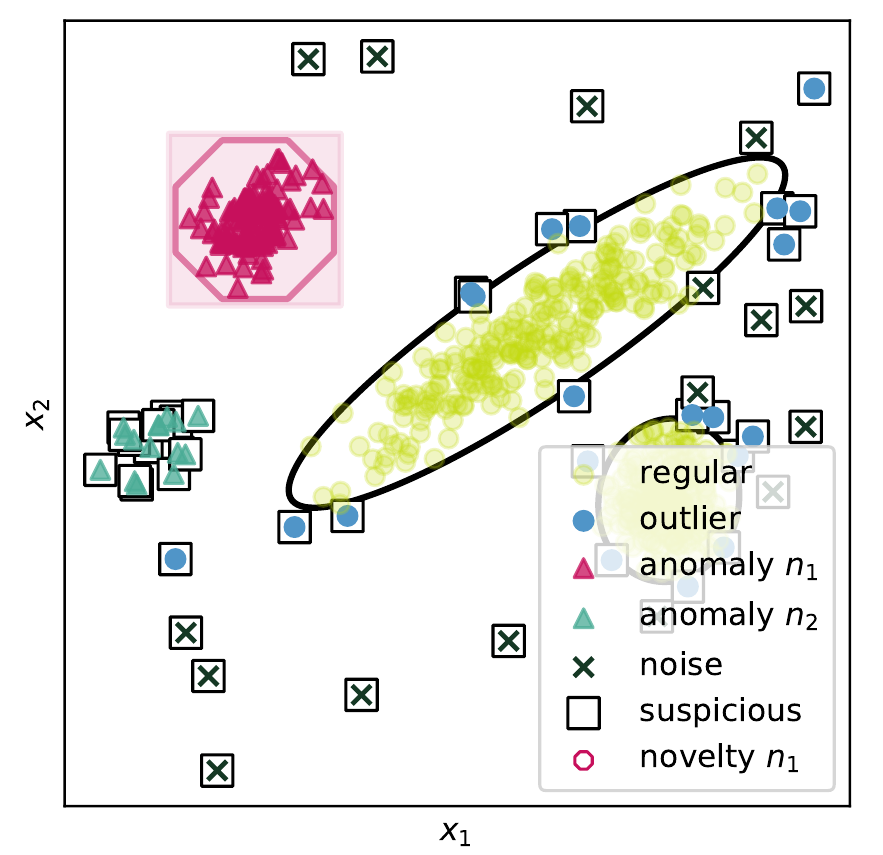
\includegraphics[width=0.8\textwidth]{images/gruhl_anomaly_definition.png}
  \caption{Classification of outliers \cite[p. 54]{gruhl_novelty_2022}}
  \label{fig_anomaly_gruhl}
\end{figure}

% definiton by shape
Instead of dividing anomalies by their cause the shape of anomalies can vary in several ways. In real measurement data of any shape is possible and it is totally unpredictable \cite{schwartz_maeday_2024}. For training purposes anomaly injection is crucial. Then the anomalies are simulated as point anomalies or subsequence anomalies. Point anomalies occur once and can be global or contextual. Subsequence anomalies on the other hand change the values in a given time window or on long term. They can be divided in seasonal, shapelet and trend anomalies (see figure \ref{fig_anomaly_carla}). Seasonal and shapelet anomalies change the values in a limited time window, trend anomalies are changing all following values \cite[p. 9]{darban_carla_2024}. %Seasonal in time direction, shapelet the amplitudes
\begin{figure}[h!] % 'h!' tries to place the figure here
  \centering
  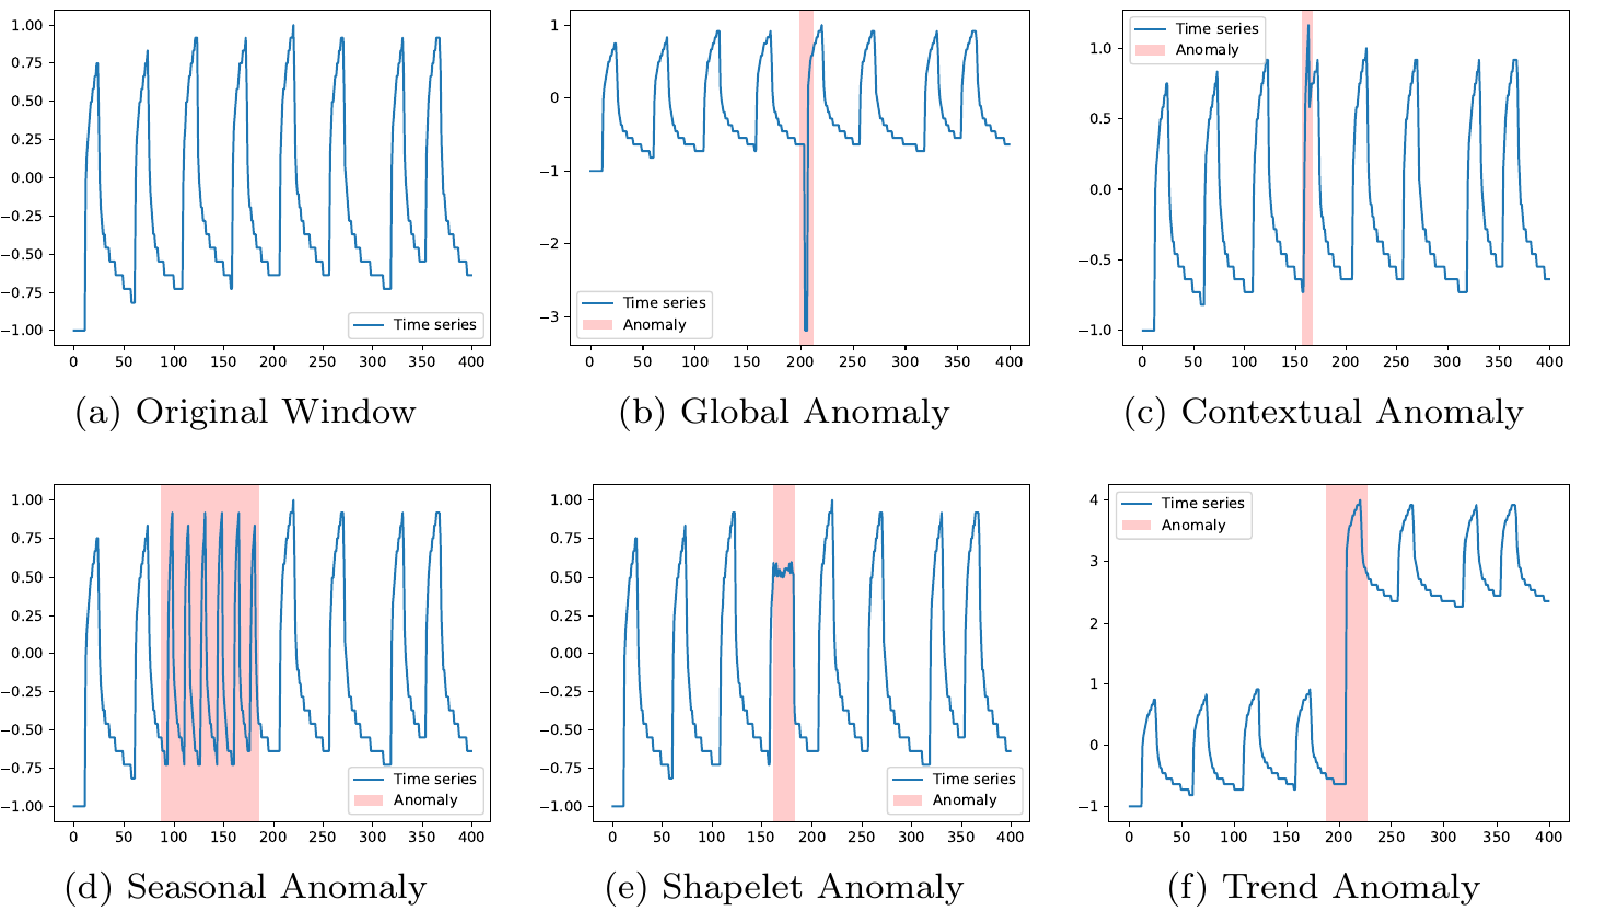
\includegraphics[width=0.8\textwidth]{images/carla_anomalies.png}
  \caption{Classification of time series anomaly types \cite{darban_carla_2024}}
  \label{fig_anomaly_carla}
\end{figure}

% definiton for this paper
In this paper we want to focus on single time events, which are in any case anomalies because they cannot form its own cluster. This defines our goal as an Anomaly Detection (AD) task.

\subsection{Zero Shot Learning}
%Definiton by Chandana
In this paper the definition made by \cite{nivarthi_unified_2022} is used. They seperate Single Task Learning, where every model is trained seperately for each task, from Multi Task Learning (MTL) where one model is trained and evaluated on several tasks. For Zero Shot Learning (ZSL) in comparison the model is trained on several tasks like in MTL but tested on completely new ones.

% Zero Shot derived from Transfer learning
Zero Shot Learning is therefore an extreme form of transfer learning. While transfer learning is the concept of transferring the knowledge and weights gained at one task using them at solving another task, Zero-Shot Learning means there are no samples for the other task. The transformation of knowledge can help solving tasks where there are few or no samples available. The gained knowledge is normally stored as representations of data. Representations which are abstract enough to not see a specific item but information about items. This also means that ZSL is only possible because additional information has been discovered during training \cite[p. 536]{goodfellow_deep_2016}.

% First zero shot detection
\cite{palatucci_zero-shot_2009} were the first to implement a successful Zero-Shot Anomaly Detection followed by \cite{socher_zero-shot_2013} who used semantic word vector representations to classify words in groups with a fully unsupervised model.

Zero-shot learning involves training a model on certain classes and then testing its ability to recognize new, unseen classes without any retraining. In the context of anomaly detection, this means the model should be able to detect types of anomalies it has not encountered during the training phase.
